\section{Performance and scaling}
\label{sec:performance}

\begin{figure}[t]
\centering
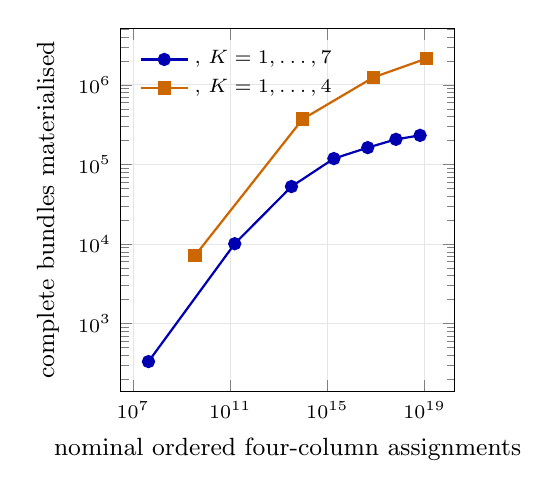
\begin{tikzpicture}
\begin{loglogaxis}[
  width=0.48\textwidth, height=6.2cm,
  xlabel={nominal ordered four-column assignments},
  ylabel={complete bundles materialised},
  legend pos=north west, legend style={font=\scriptsize, draw=none, fill=none},
  tick label style={font=\scriptsize}, label style={font=\small},
  grid=major, grid style={gray!20}]
\addplot[mark=*, thick, blue!70!black] coordinates {
  (4.30e7,334) (1.53e11,10097) (3.32e13,52800) (1.85e15,118577)
  (4.59e16,162761) (6.65e17,206847) (6.57e18,231946)};
\addlegendentry{$\Xa$, $K=1,\dots,7$}
\addplot[mark=square*, thick, orange!80!black] coordinates {
  (3.49e9,7122) (9.54e13,371214) (7.98e16,1245469) (1.22e19,2142164)};
\addlegendentry{$\Xb$, $K=1,\dots,4$}
\end{loglogaxis}
\end{tikzpicture}\hfill
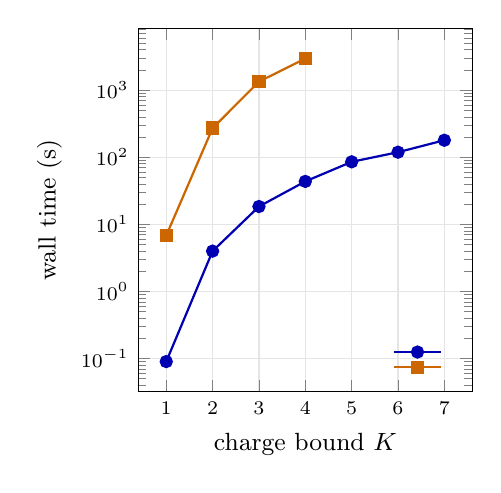
\begin{tikzpicture}
\begin{semilogyaxis}[
  width=0.48\textwidth, height=6.2cm,
  xlabel={charge bound $K$}, ylabel={wall time (s)},
  legend pos=south east, legend style={font=\scriptsize, draw=none, fill=none},
  tick label style={font=\scriptsize}, label style={font=\small},
  grid=major, grid style={gray!20}, xtick={1,2,3,4,5,6,7}]
\addplot[mark=*, thick, blue!70!black] coordinates {
  (1,0.09) (2,3.99) (3,18.42) (4,43.62) (5,85.44) (6,118.88) (7,179.15)};
\addlegendentry{$\Xa$}
\addplot[mark=square*, thick, orange!80!black] coordinates {
  (1,6.8) (2,271.6) (3,1338.8) (4,2960.2)};
\addlegendentry{$\Xb$}
\end{semilogyaxis}
\end{tikzpicture}
\caption{Left: the number of complete bundles the search actually builds against
the nominal size of the domain. Across eleven orders of magnitude in the domain
the materialised set grows by less than three, because the monotone rules prune
entire subtrees. Right: wall time on a single core ($\Gam=\Z_2$, complete slope
rule, bitset-indexed engine; the $\Xa$, $K=4$ point drops to 28.8\,s with the dual
slope decision).}
\label{fig:scaling}
\end{figure}

\Cref{fig:scaling} summarises the scaling. Three observations. First, the
materialised search space is essentially decoupled from the nominal one: on
$\Xa$ the nominal domain grows by a factor $1.5\times10^{11}$ from $K=1$ to $K=7$
while the bundles built grow by $7\times10^{2}$. Second, memory is not the
binding resource at this scale: peak resident memory is 189\,MiB at $\Xa$, $K=7$
and 706\,MiB at $\Xb$, $K=4$. Third, the cost of a node falls with depth because
of the dual slope decision (\cref{prop:dual}), so the dominant cost moves from
the slope test to enumeration as the search deepens.

Every escalation was preceded by a pilot and a written estimate: a $K=4$ pilot
on 8 roots predicted 110--450\,s against an actual 204.8\,s (before indexing),
and the $\Xb$ orbit counts at $K=2,3,4$ were predicted exactly from the
published catalog before the runs. For the downstairs stage, computing the
$\Gam$-representation on a 120-dimensional ambient cohomology group takes under
a second with the exact rational rank path.

The whole test suite---unit, differential (brute force against the split search
under all three slope-rule settings), certificate-replay and regression
tests---runs in about 30 seconds.
